\documentclass[output=paper]{langsci/langscibook} 
\author{Melanie Uth\affiliation{Universität zu Köln}}
\title{F0 contours in data from picture-based elicitation experiments: Evidence from contrastive cleft sentences in Yucatecan Spanish}
\shorttitlerunninghead{F0 contours and picture-based elicitation designs}
% \chapterDOI{} %will be filled in at production '
% Keywords: Picture-based elicitation, information structure, pragmatics, intonation
 
\abstract{
This paper discusses semi-spontaneous picture-based experiments that are de\-signed to elicit the syntactic and prosodic realization of different focus types (broad, narrow, and contrastive) in Spanish (cf. e.g. \citealt{Gabriel2007,Gabriel2010article,Heidinger13,Heidinger14,Feldhausen2014}). Data from a picture-based elicitation experiment carried out in Yucatán, Mexico with slightly differing elicitation materials is examined. Findings suggest that, among other things, the intonational realization of certain elicited focus constructions depends on the exact design of the experiment, especially regarding the complexity of the elicitation story and the kind of elicitation questions.
}
\maketitle

\begin{document}
\label{chap:uth}

\section{Introduction} 
\label{sec:uth:1}
The main goal of the present paper is to compare the intonation of contrastive cleft sentences taken from a three-part comparative picture-based elicitation \linebreak study. The comparative study is composed of three designs that differ slightly with respect to the pragmatic appropriateness of the picture stimuli and the accompanying questions.

Picture-based elicitation experiments are used to elicit semi-spontaneous \linebreak speech and obtain inter-individually comparable, semi-spontaneous data by large\-ly controlling for \\
(i) the segmental make-up of the target words/utterances and \\
(ii) the pragmatic context. \\
The basic architecture consists of a series of pictures shown to the informants on a screen and a series of questions relating to these pictures, intended to trigger the realization of certain kinds of information structural categories. Instead of isolated pictures, various authors such as \citet{Gabriel2007,Gabriel2010article,Heidinger13,Heidinger14,Feldhausen2014} use short picture stories designed to enhance the naturalness of the utterance contexts (cf. \sectref{sec:uth:2}).

This latter kind of picture-based elicitation has several advantages compared to previous elicitation experiments as they are located in the middle of the ``authenticity continuum" of data elicitation. For one thing, the speech of the participants is generally more lively, authentic, and diverse compared to the output elicited by e.g. reading tasks or stylized intonation studies (recoverable intonation patterns of e.g. vocatives, salutations of ritual speech, etc.). For another thing, the picture-based elicitation experiments provide much more comparable data than spontaneous recordings, since several speakers do more or less the same thing. Finally, the core idea of picture-/short story-based elicitation is to control the elicited utterances with respect to length, segmental make-up, pragmatic contexts, and illocutionary acts or propositional attitudes as closely as possible. However, as will be argued below, the control for pragmatic contexts and propositional attitudes is one of the main challenges of picture-based elicitation experiments. This paper takes a skeptical position with regard to the reach of the pragmatic control of picture- and short story-based elicitation experiments. It is argued that the design contains several ‘pragmatic mismatches’ which might impede the participants from properly performing the language task as intended, meaning that there are reasons to doubt that the corresponding production data can be unambiguously coded for pragmatic contexts and/or propositional attitudes. Furthermore, we report on a comparative picture-based elicitation experiment for Yucatecan Spanish composed of three designs which differ slightly with respect to the pragmatic appropriateness of the picture stimuli and the accompanying questions. Our analysis of the production data obtained by means of these materials suggests that, at least in the case of Yucatecan Spanish contrastive cleft sentences, the intonational realization of the constructions highly depends on the exact design of the elicitation experiment. It is argued that this difference in intonational realization is further evidence of the need for more elaborated contexts and unequivocal triggers in the realm of focus elicitation. 

The outline of the paper is as follows: \sectref{sec:uth:2} presents the core design of the picture-based elicitation design initially used by \citet{Gabriel2007} and discusses the pragmatic mismatches alluded to above (\sectref{sec:uth:2.1}). Furthermore, it presents the comparative picture-based elicitation experiment with three pragmatically varying conditions (\sectref{sec:uth:2.2}). \sectref{sec:uth:3} delineates the core characteristics of the prosodic realization of contrastive focus in Yucatecan Spanish according to \citet{GriceUth15} and \citet{Uth16}. \sectref{sec:uth:4} presents the differences in the prosodic realization of contrastive cleft sentences that were elicited by means of the three-part comparative picture-based elicitation experiment, and \sectref{sec:uth:5} summarizes the main results and conclusions.


\section{Picture-based elicitation experiments and propositional attitudes}
\label{sec:uth:2}
\subsection{Design initially proposed by \citet{Gabriel2007}}
\label{sec:uth:2.1}
In this section, we describe the short story-based elicitation design first used by \citet{Gabriel2007} to investigate the realization of different focus categories in declarative sentences produced by speakers of different varieties of Spanish. We then comment on the pragmatic appropriateness of the design with respect to the propositional attitudes the participants are expected to adhere to when answering the accompanying wh-questions.

Gabriel’s \citeyearpar{Gabriel2007} experiment consists of two steps. First, short picture stories, each composed of four pictures, are shown to the informants in order to introduce the relevant referents and the scene which the informants will be asked about. Afterward, the same pictures are repeatedly shown to the informants again, each picture being accompanied by a written \textit{wh}- or \textit{yes/no}-question asking about a subject or object referent that was introduced before. Contrastive / corrective statements are elicited by means of several \textit{yes / no}-questions of the type \textit{¿\textbf{Julia} compra el diario en el kisco, verdad?} (‘Julia buys the newspaper at the kiosk, right?'). The participants are told to imagine that the questions are being asked by interlocutors that do not know each other and that are entirely unfamiliar with the questions that were asked before. Furthermore, the participants are asked to answer using complete sentences, and in order to emphasize this request, they are told that the data will be used to train learners of Spanish as a second language. The 18 Hispanic participants interrogated by \citet{Gabriel2007,Gabriel2010article} are from different regions of Spain (14 participants) and Latin America (4 participants) and are graduate students or university staff.

%\begin{table}
% \begin{tabularx}{\textwidth}{XXXX}
% \lsptoprule
% (Ia.) & 
% 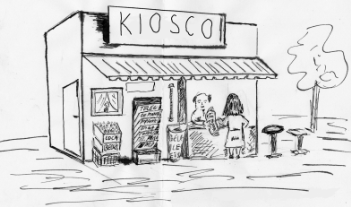
\includegraphics[width=\textwidth]{figures/UTH-img1.png} & {(IIa.)} & 
% 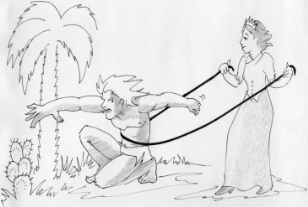
\includegraphics[width=\textwidth]{figures/UTH-img2.png}\\
% \multicolumn{2}{p{5cm}}{{\textit{María compra el diario en el kiosco.} }
% 
% ‘María buys the newspaper at the kiosk.’} & \multicolumn{2}{p{5cm}}{{\textit{Blancanieves secuestra a Tarzán...}}
% 
% ‘Snow White kidnaps Tarzan...’}\\
% (Ib.) & 
% 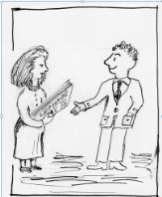
\includegraphics[width=\textwidth]{figures/UTH-img3.png} & {(IIb.)} & 
% 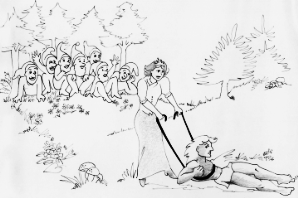
\includegraphics[width=\textwidth]{figures/UTH-img4.png}\\
% \multicolumn{2}{p{5cm}}{\textit{Después se lo da a su hermano.}\\
% ‘Shortly after, she gives it to her brother.’} & \multicolumn{2}{p{5cm}}{\textit{.. y se lo entrega a los siete enanitos.}
% 
% ‘... and hands him over to the Dwarfs.’}\\
% (Ic.) & 
% 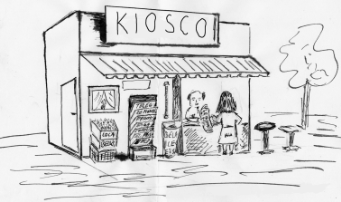
\includegraphics[width=\textwidth]{figures/UTH-img5.png} & (IIc.) & 
% 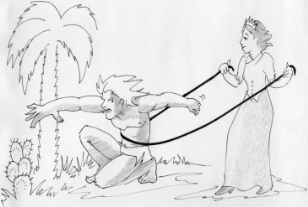
\includegraphics[width=\textwidth]{figures/UTH-img6.png}\\
% \multicolumn{2}{p{5cm}}{{\textit{¿}\textbf{\textit{Julia}} \textit{compra el diario en el kisco, verdad?}}
% 
% ‘Julia buys the newspaper at the kiosk, right?’} & \multicolumn{2}{p{5cm}}{{\textbf{\textit{La Bella Durmiente}} \textit{secuestra a Tarzán, verdad?}}
% 
% ‘Sleeping Beauty kidnaps Tarzan, right?’}\\
% \lspbottomrule
% \end{tabularx}

%\caption{Experimental design of \citet{Gabriel07} with choice of two correction seeking \textit{yes/no}-questions}
%\label{tab:uth:1}
%\end{table}

Among other things, the inquiry is designed to elicit contrastive focus utterances by means of the above-cited \textit{yes/no}-questions. As far as intonation is concerned, contrastively and non-contrastively focused constituents in the data of \citet{Gabriel2007} are uniformly marked by means of the most common contrastive accent of Standard Spanish, i.e. L+H*, in the conventional Sp\_ToBI notation (\citealt[283]{Gabriel2007}, \citealt{Beckman.2002}). Regarding syntactic realization, Gabriel's \citeyearpar{Gabriel2007} results confirm several judgements stated in the literature, e.g. the fact that contrastive focus in Spanish can in principle be realized by means of the following syntactic constructions: emphatic stress assignment (\ref{ex:uth:1}a), focus fronting (\ref{ex:uth:1}b.), \textit{p}-movement (\ref{ex:uth:1}c.), clefting (\ref{ex:uth:1}d,e) or other syntactic strategies (\ref{ex:uth:1}f). The examples are adapted from \citet[377]{GutierrezBravo08}, \citet[20]{Zubizarreta98}, \citet[4229,4242]{Zubizarreta99} and \citet[283]{Gabriel2007}.

\ea%1
    \label{ex:uth:1}
    \ea{}  [\textsubscript{Fc} JUAN] comió una manzana (no Pedro). 
    \ex{}  [\textsubscript{Fc} MANZANAS] compró Pedro (y no peras / PERAS). 
    \ex{}	La Bella Durmiente entrega a Tarzan a los siete enanitos, verdad? \\
      – No, se lo entrega [\textsubscript{Fc} BLANCANIEVES].
    \ex La que votó por Pedro fue [\textsubscript{Fc} Luz / LUZ].
    \ex Fue [\textsubscript{Fc} MANZANAS] lo que compró Pedro (y no peras / PERAS).
    \ex Julia le da un diario a su hermano, verdad?\\
      – No, Es [\textsubscript{Fc} Blancanieves / BLANCANIEVES]. 
      \z
      \z

However, the most important benefit of this line of research is its extensive experimental background, which enables \citet{Gabriel2007} to contribute entirely new and rewarding insights to several discussions concerning Spanish word order. Note that previous studies on Spanish word order and sentence intonation relied entirely either on reading tasks (e.g. \citealt{Dominguez04,Face2002,Hualde2005}) or introspective data (e.g. \citealt{Zubizarreta98,Zubizarreta99}), meaning that \citet{Gabriel2007} was the first author to introduce the important issues of (true) variability and usage frequency into the discussion. More concretely, according to Gabriel's data, non-contrastively focused subjects are realized 100\% \textit{in situ} and marked prosodically with L+H*, in the case of “constructions with one or several entire objects-DPs” (\citealt[290]{Gabriel2007}, e.g.‚ Who gives her brother the paper?\textit{– ${\surd}$ [María]\textsubscript{F} le da el diario a su hermano.}, \citealt[289]{Gabriel2007}), a result which is diametrically opposed to the syntactic research of \citet{Zubizarreta98,Zubizarreta99} and others.

A second important result of \citet{Gabriel2007} is that there is no real empirical evidence that would corroborate the usage of the \textit{foco antepuesto} constructions, such as the one cited under (\ref{ex:uth:1}b), by native speakers of Spanish. On the contrary, there is not a single instance of this type of construction in the production data of \citet[285]{Gabriel2007}. Furthermore, when asked to read out the corresponding constructions such as (\ref{ex:uth:2}a), more than half of the informants either pronounced the sentences with a dubitative/inquiring contour or they used the prosodic contour characteristic of topic-comment constructions (ibid.). One speaker even introduced a resumptive pronoun into his utterance (\ref{ex:uth:2}b). From such data, we may conclude that the constructions are either judged as grammatically deviant or reinterpreted as topicalizations by the corresponding informants.

\ea%2
    \label{ex:uth:2}
    \ea   ¡No! Un [\textsubscript{Fc} diario] compró María en el kiosco.
    \ex{}   [El diario]\textsubscript{i} se lo\textsubscript{i} dio a su hermano. \citep[285]{Gabriel2007}
\z
\z

It is true, however, that the informants of \citet{Gabriel2007} accepted the contrastive \textit{foco antepuesto} to a fairly high degree in the corresponding perception experiments, meaning that it seems to be an acceptable, albeit marginal, option in Spanish.

Against this background, the contribution of Gabriel's \citeyearpar{Gabriel2007} experiments is unquestionable. Nevertheless, from a pragmatic point of view, the elicitation design carries with it several pragmatic mismatches which lead us to suspect that the participants are not necessarily performing the language task as intended. The first problem relates to the fact that the four visual stimuli described above, displaying four simple activities, serve as a basis for an elaborate series of questions from unknown and unspecified questioners. This is to say that even if the speakers assume that the questioners do not know the protagonists in the pictured scenes, their motivation for asking all these very similar questions remains unclear. Thus, there is a pragmatic mismatch between the simplicity and vagueness of the visual stimuli on the one hand and the multitude of information-seeking questions on the other. 

The second pragmatic problem is that the participants are repeatedly confronted with obvious information, whereas the focus structure of the intended utterances suggested by the accompanying questions requires them to provide new (or ‘newsworthy’, \citealt{Baumann2006}) information. To a certain degree, this is a problem for any elicitation experiment that requires participants to answer focusing questions asking for information related to previously introduced referents. However, in the elicitation design at hand, this problem is increased by two further pragmatic mismatches. 

The first additional problem relates again to the vague communicative setting, which does not fit the specific Information Structures that are intended to be elicited by means of the questions: In the context of a scene such as the one displayed in visual stimuli described above, there is no pragmatic need to call into question the (obvious) information conveyed by the picture stimuli by using a correction-seeking yes/no-question, and it is difficult to imagine a scenario in which the unknown interlocutors could not properly relate the pictures to the referents in the extra-linguistic world \textit{without} asking for the relevant information.

The second additional problem relates to the pragmatic clash between the undefined status of the unknown questioners and their inexplicable familiarity with the referents, the latter being suggested by the fact that the referents are introduced into the discourse by using their first names. The pragmatic problem is the following. On the one hand, the communicative setting implies that the unknown questioners do not know the protagonists (cf. above). Moreover, it is probable that the unspecified status of the questioners and the large number of questions further strengthen this interpretation indirectly. On the other hand, from the participants’ point of view, if the undefined questioners did not know the protagonists of the short stories, they could not refer to them by their first or proper names. 

In short, the simplistic stimuli probably implicitly urge the participants of the elicitation study to pragmatically enrich the communication. At the same time, the clash between the unknown questioners’ unfamiliarity with the protagonists on the one hand and their use of first names when referring to them on the other probably impedes the participants from performing the language task as intended. This means that, very probably, the corresponding production data cannot be unambiguously controlled for illocutionary acts or propositional attitudes. A propositional attitude may be defined as a ``psychological attitude towards a state of affairs (…) expressed by a proposition" (\citealt[47]{Moraes12}). This kind of speaker attitude has been shown to highly influence the prosodic realization of questions and assertions in different languages, such as e.g. Catalan (\citealt{Vanrell2014evidentiality,Roseano2015epistemic,Borras-Comes2015}), Brazilian Portuguese (\citealt{Moraes11,Moraes12}), and Mexican Spanish (\citealt{FliessbachReich14}). Hence, it might be reasonable to stick to elicitation designs with concrete and explicit communicative settings in order to be able to control as closely as possible for the attitudes of the participants toward the propositional content of their utterances. 
 
\subsection{Alternative design and comparative elicitation experiment}
\label{sec:uth:2.2}
In order to empirically verify the methodological concerns described above, we designed a three-part elicitation experiment based on those of \citet{Gabriel2007}.\footnote{I am grateful to Christoph Gabriel for sharing the original slides of the 2007 inquiry, and to Henrike Rödiger for the design of the further stimuli.} In one third of the queries, which were conducted with five participants, we closely followed the design of \citet{Gabriel2007} by copying (i) the picture stimuli, (ii) the elicitation questions, and (iii) the instructions to make sure that the same conditions held in both elicitation settings. In the second third of the queries, conducted with five other participants, we likewise followed the design of \citet{Gabriel2007}. However, we introduced the referents by means of indefinite noun phrases instead of proper names. We hypothesized that this would avoid the clash between the unknown questioners and their inexplicable familiarity with the protagonists suggested by using first names, and thus facilitate the intended behavior on the part of the speakers. Crucially, in the last third of the queries, which were conducted with five other informants, we modified the pictorial stimuli in order to base our query in a more elaborate and better-defined communicative setting. The prosodic analysis of the contrastive cleft sentences that were obtained in each of the three conditions is presented in \sectref{sec:uth:4}. In the following, we will first delineate the pragmatic differences between the copied and the newly designed picture-based elicitation designs.

%Tables \ref{tab:uth:2} and \ref{tab:uth:3} list the newly designed short stories used to introduce the referents and to create communicative settings appropriate for the subsequent questioning. 


\begin{table}
\begin{tabularx}{\textwidth}{p{5cm}p{6cm}}
\begin{minipage}[t]{5cm}(Ia.)
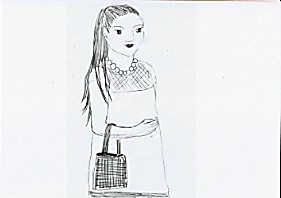
\includegraphics[width=5cm]{figures/UTH-img7.png}
\end{minipage}& \begin{minipage}[t]{6cm}
\ \\
\textit{Ella es Aruma Hernández Casas}.\\
{‘This is Aruma Hernández Casas.’}
\end{minipage}\\
\ \\
\begin{minipage}[t]{5cm}(Ib.)
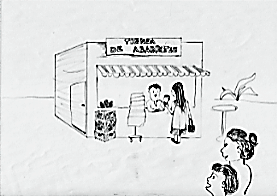
\includegraphics[width=5cm]{figures/UTH-img8.png}
\end{minipage}& \begin{minipage}[t]{6cm}
\ \\
\textit{Aruma compra un periódico en una tienda, y una conocida con su hija la están mirando desde lejos.}\\
{‘Aruma buys a newspaper in a kiosk, and a friend with her daughter are looking at her from a distance.’}
\end{minipage}\\
\ \\
\begin{minipage}[t]{5cm}(Ic.)
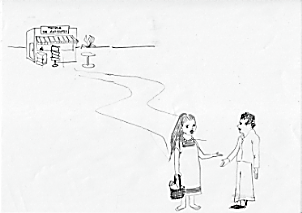
\includegraphics[width=5cm]{figures/UTH-img9.png}
\end{minipage}& \begin{minipage}[t]{6cm}
\ \\
\textit{Después, Aruma encuentra a su amigo Don Hernando y dan un paseo en un parque cercano.}\\
{‘Afterwards, Aruma encounters her friend Don Hernando. They go for a walk in a near public park.’}
\end{minipage}\\
\ \\
\begin{minipage}[t]{5cm}(Id.)
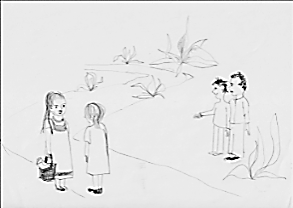
\includegraphics[width=5cm]{figures/UTH-img10.png}
\end{minipage}& \begin{minipage}[t]{6cm}
\ \\
\textit{En el parque, encuentran a unos amigos y se paran un rato a platicar con ellos.}\\
{‘In the park, they encounter some friends and they stay a bit in order to have a conversation.’}
\end{minipage}\\
\ \\
\end{tabularx}
 \caption{\label{tab:uth:1} Experimental design of elaborate elicitation study (condition 3), picture story 1.}
\end{table}

\begin{table}
\begin{tabularx}{\textwidth}{p{5cm}p{6cm}}
\begin{minipage}[t]{5cm}(Ie.)
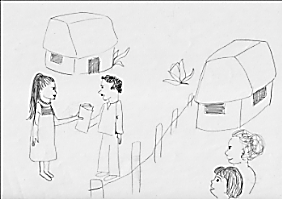
\includegraphics[width=5cm]{figures/UTH-img11.png}
\end{minipage}& \begin{minipage}[t]{6cm}
\ \\
\textit{Luego, Aruma acompaña a Don Hernando a casa y le da el periódico. Sus vecinos los están mirándo desde su jardín.}\\
{‘Aruma walks home with Don Hernando and she gives him the newspaper, Don Hernando’s neighbors being in their backyard looking at them.’}
\end{minipage}\\
\ \\
\begin{minipage}[t]{5cm}(If.)
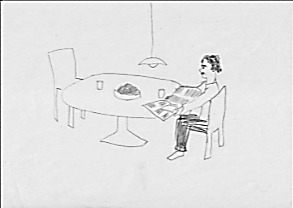
\includegraphics[width=5cm]{figures/UTH-img12.png}
\end{minipage}& \begin{minipage}[t]{6cm}
\ \\
\textit{Don Hernando entra a su casa, prepara la cena y espera a su hermana, leyendo el periódico.}\\
{‘Don Hernando enters his home, prepares the dinner and waits for her sister, reading the newspaper.’}
\end{minipage}\\
\ \\
\begin{minipage}[t]{5cm}(Ig.)
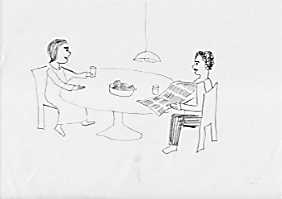
\includegraphics[width=5cm]{figures/UTH-img13.png}
\end{minipage}& \begin{minipage}[t]{6cm}
\ \\
\textit{Por fin, llega su hermana y empiezan a cenar.}\\
{‘Finally his sister gets home and they have dinner.’}
\end{minipage}\\
\ \\
\end{tabularx}
\end{table}



\begin{table}
\begin{tabularx}{\textwidth}{p{5cm}p{6cm}}
\begin{minipage}[t]{5cm}(IIa.)
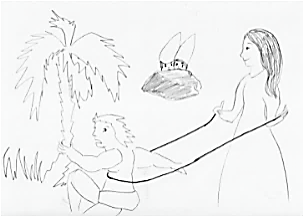
\includegraphics[width=5cm]{figures/UTH-img14.png}
\end{minipage}& \begin{minipage}[t]{6cm}
\ \\
\textit{Blancanieves secuestra a Tarzán, y dos enanitos los están mirando de detrás de una roca.}\\
{‘Snow White kidnaps Tarzan, two dwarfs hiding behind a rock and looking at them.’}
\end{minipage}\\
\ \\
\begin{minipage}[t]{5cm}(IIb.)
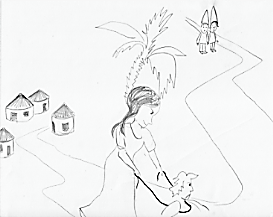
\includegraphics[width=5cm]{figures/UTH-img15.png}
\end{minipage}& \begin{minipage}[t]{6cm}
\ \\
\textit{Después, Blancanieves entrega a Tarzán al pueblo de los Siete Enanitos}, …\\
{‘Afterwards, Snow White brings Tarzan to the village of the Seven Dwarfs, ...’}
\end{minipage}\\
\ \\
\begin{minipage}[t]{5cm}(IIc.)
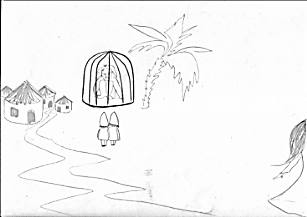
\includegraphics[width=5cm]{figures/UTH-img16.png}
\end{minipage}& \begin{minipage}[t]{6cm}
\ \\
\textit{… lo encierra en un huacal y vuelve a salir para colectar hongos para la cena.}\\
{‘She locks him up in a cage and leaves the village in order to collect mushrooms for the dinner.’}
\end{minipage}\\
\ \\
\begin{minipage}[t]{5cm}(IId.)
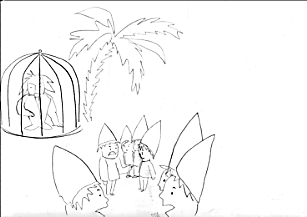
\includegraphics[width=5cm]{figures/UTH-img17.png}
\end{minipage}& \begin{minipage}[t]{6cm}
\ \\
\textit{Luego, regresan los cinco enanitos restantes a su pueblo. Están todo asustados por la enorme criatura en el huacal.}\\
{‘Shortly after, the remaining five dwarfs come back to the village being totally scared by the huge creature sitting in the cage.’}
\end{minipage}\\
\ \\
\end{tabularx}
 \caption{\label{tab:uth:2} Experimental design of elaborate elicitation study (condition 3), picture story 2.}
\end{table}

During the elicitation sessions, the participants were told that the pictures would be shown to them once again, but that the second time they would be accompanied by speech balloons. Furthermore, the participants were told that they were supposed to fill in the balloons by giving contextually appropriate answers. Finally, as in the context of Gabriel’s \citeyearpar{Gabriel2007,Gabriel2010article} experiments, they were asked to answer using complete sentences and to speak as naturally as possible.

For the present purposes, the most important modification of the alternative design compared to the previous one boils down to the introduction of the above-displayed specific communicative settings, in which correction-seeking \textit{yes/no}-questions can be asked in a more meaningful manner. Two of the correction-seeking questions which form part of our modified elicitation design are shown in \tabref{tab:uth:3}. It is obvious that the alternative design circumvents the abovementioned pragmatic mismatches (i) by providing more complex picture stories, an unambiguous communicative setting, and non-obvious questions, and (ii) by the fact that the (explicitly defined) questioners are obviously familiar with the referents whom they refer to by their proper names.

\begin{table}
\begin{tabularx}{\textwidth}{p{5cm}p{6cm}}
\begin{minipage}[t]{5cm}(IIIa.)
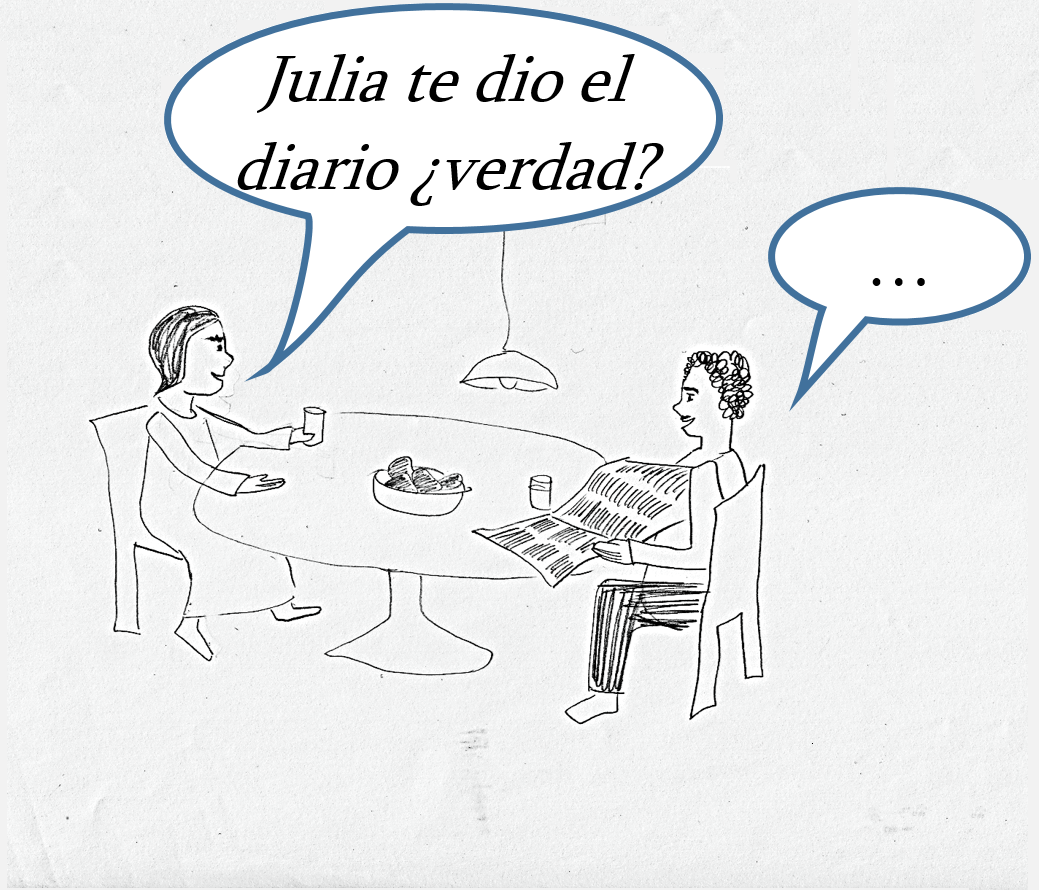
\includegraphics[width=5cm]{figures/UTH-img18new.png}
\end{minipage}& \begin{minipage}[t]{6cm}
\ \\
{‘Julia gave the newspaper to you, right’}
\end{minipage}\\
\ \\
\begin{minipage}[t]{5cm}(IIIb.)
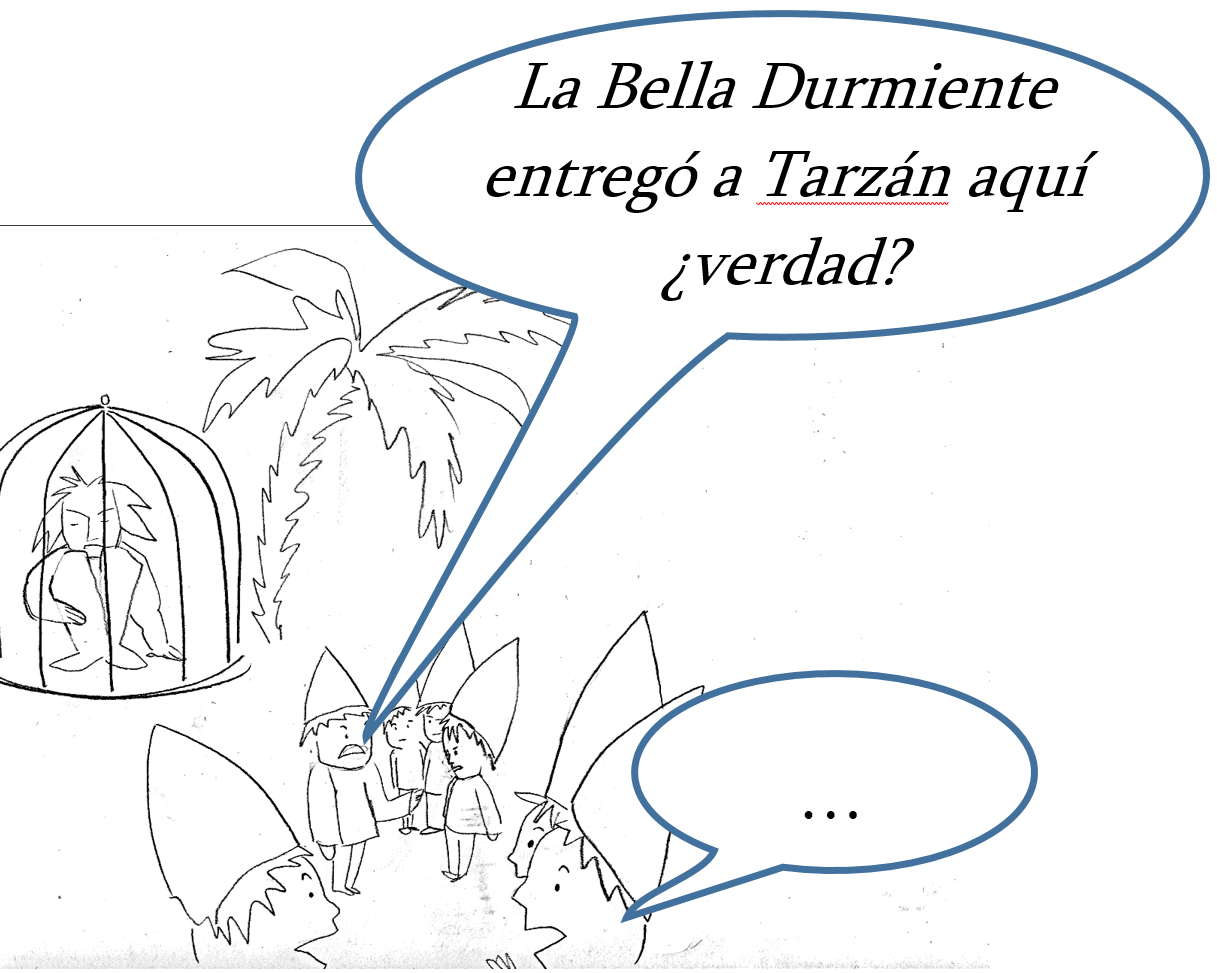
\includegraphics[width=5cm]{figures/UTH-img19.png}
\end{minipage}& \begin{minipage}[t]{6cm}
\ \\
{‘Sleeping Beauty brought Tarzan to our village, right?’}
\end{minipage}\\
\ \\
\end{tabularx}
\caption{Examples of two correction-seeking yes/no-questions from the elaborate elicitation design (condition 3).}
\label{tab:uth:3}
\end{table}


The three sub-studies were performed with different participants since recording the same participants with the three similar elicitation designs would have had psychological priming and repetition effects. However, all 15 participants were female monolingual speakers of Yucatecan Spanish who had lived on the Yucatán peninsula since birth. At the time of the experiments, they were 19 to 22 years old and about to complete 12\textsuperscript{th} grade at the local high school. Moreoever, these pupils likewise formed a largely homogeneous group from a sociolinguistic viewpoint. They were all born in the north-eastern part of the Yucatán peninsula (Cancún, Valladolid, Felipe Carrillo Puerto, Cozumel Island, Chetumal) and moved to Felipe Carrillo Puerto during childhood or early adolescence. All of them went to the same high school and interacted with each other daily at the time of the recording, and they had a similar social background as far as their family and cultural background (e.g. leisure activities) was concerned. 

\section{Contrastive focus marking in Yucatecan Spanish}
\label{sec:uth:3}
In order to properly assess the main prosodic difference between the cleft sentences obtained in the comparative picture-based elicitation experiments, it is necessary to mention two interrelated prosodic particularities of Yucatecan Spanish (YS) (cf. the elicitation-based study of \citealt{Uth16}; also \citealt{GriceUth15}). In what follows, we will first delineate the methodology employed by \citet{Uth16} (\sectref{sec:uth:3.1}) before summarizing the results with regard to the prosodic realization of contrastive focus in YS  (\sectref{sec:uth:3.2}). 
  
\subsection{Methodology}
\label{sec:uth:3.1}
The data for the present analysis stems from one elicitation study and one grammaticality judgment test, which were run in August 2012 and March 2013 in Quintana Roo, Mexico. In what follows, we present the sub-corpora in three separate subsections: (i) participants, (ii) materials and procedure, and (iii) results (only first sub-corpus).

\subsubsection{Data base 1: ELIC01}
\label{sec:uth:3.2}

\begin{enumerate}[(i)]
\item{Participants}

Ten bilingual speakers (nine women and one man) took part in the first study, subsequently abbreviated as ELIC01. The ten participants are YS speakers between the ages of 20 and 70 with at least some degree of proficiency in Yucatec Maya (YM; cf. below) and have lived on the Yucatán peninsula since birth. Five participants are Spanish-dominant, as established by the following criteria: (1) the participants describe themselves as native speakers of YS. (2) YS was the language they had used in the home they lived in as children and adolescents. (3) YS is the language the participants use in daily life in all contexts. (4) The participants have bilingual (YS/YM) parents, understand YM and might be able to speak some simple phrases, but they very rarely communicate in YM in daily life, if at all. The remaining five speakers are balanced bilinguals. (1) They describe themselves as bilingual from birth on. (2) They have bilingual or YM-dominant parents. (3) They had used both languages in the home they lived in as children and adolescents. (4) They use both languages in their daily life in all contexts. 

\item{Materials and procedure}

ELIC01 is based on an elicitation study consisting of twenty cartoon pictures accompanied by questions. The questions are designed to elicit broad focus constructions (20x) as well as contrastively focused main verbs (10x) and contrastively focused subjects (10x). Each picture was shown twice to each informant – once to elicit broad focus and once to elicit contrastive focus on the verb (10x) or on the subject (10x). This means that each participant answered 40 questions pertaining to one of the three experimental conditions, and each of the different focus conditions served as a filler for the two remaining conditions.

%\begin{table}
%\todo[inline]{What is the copyright status of these drawings?}
%\begin{tabularx}{\textwidth}{lQQ}
%I. &\vspace*{0pt} 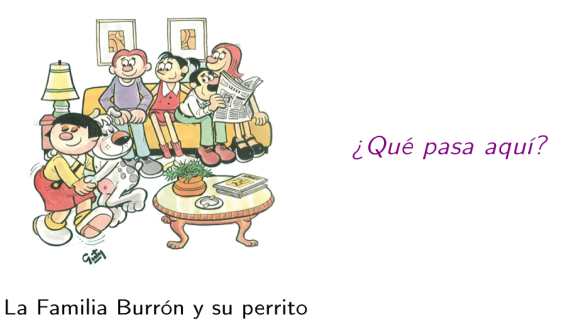
\includegraphics[width=4cm]{figures/UTH-img20.png} & 
%    Broad focus (n=20)\newline
%    \textit{¿Qué pasa aquí?}\newline 
%    ‘What happens?’\\
%IIa. &\vspace*{0pt}   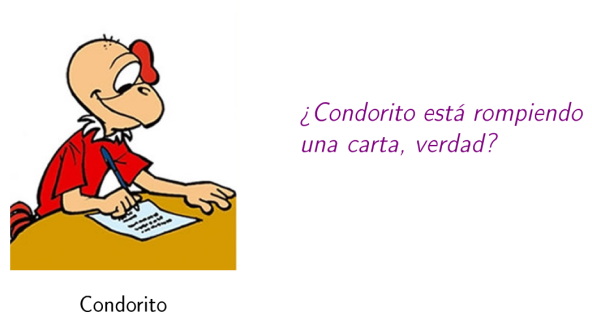
\includegraphics[width=4cm]{figures/UTH-img21.png} & 
%    Contrastive focus on verb (n=10)\newline 
%    \textit{¿Condorito está rompiendo und carta, verdad?}\newline 
%    ‘Condorito is destroying a letter, right?’ \\
%IIb. &\vspace*{0pt}   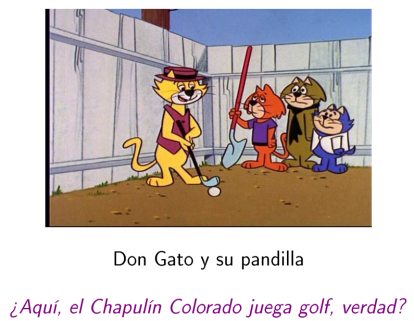
\includegraphics[width=4cm]{figures/UTH-img22.png} &
%    Contrastive focus on subject (n=10)\newline 
%    \textit{¿Aquí, el Chapulín Colorado juega golf, verdad?}\newline 
%    ‘In this picture Chapulín Colorado plays golf, right?’\\
%\end{tabularx} 
%\caption{Experimental design of ELIC01}
%\label{tab:uth:5}
%\end{table}

The pictures were shown to the participants on a screen and accompanied by oral questions, with the question and picture being presented simultaneously. This design was preferred to more complex designs since participants' output is still more uniform as regards the focus types (20x broad vs. contrastive). Obviously, it is true that this design is not pragmatically complex either. To the contrary, the participants were required to answer 2 times 20 pragmatically equivalent questions. Note that the drawbacks of the above-mentioned previous elicitation designs do nevertheless not apply to these stimuli since the participants are not asked to perform a previously defined language task. Instead, they were only required to use e.g. contrastively focused constituents in order to properly describe what they saw in the picture stimuli while answering the corresponding yes/no-questions. 

The pictures and their associated questions were randomized manually in such a way that there were no more than two pictures of the same condition occurring consecutively. The interviews were conducted by a local field work assistant in order to avoid distracting effects of social distance, foreigner talk, or linguistic convergence. The participants were told to avoid answers consisting of only one constituent, but to otherwise feel free regarding the phrasing of their answers. 


\item{Results}

While the broad focus questions were exclusively answered by means of SV(O/XP) sentences (\ref{ex:uth:3}a.,\ref{ex:uth:3}b.), verb contrastive focus was realized by means of in situ verbs in sentence-medial or -final position (\ref{ex:uth:3}c.,\ref{ex:uth:3}d.), and subject contrastive focus was realized by means of four different constructions: subject cleft sentences of the form \textit{esSque} (\ref{ex:uth:3}e.), gerundive sentences of the form \textit{esSger} (\ref{ex:uth:3}f.), existential ascriptions of the form \textit{esS} (\ref{ex:uth:3}g.), and preverbal subjects which, according to our hypothesis, occupy the same position as the subjects in the broad focus condition (\ref{ex:uth:3}h.).


\ea\label{ex:uth:3}
  \ea  {} [\textsubscript{F} Condorito está practicando futból.]
     \glt ‘Condorito is playing soccer.’ (ELIC01\_GGSM\_B15)
    \ex{} [\textsubscript{F} \textit{El Chavo del Ocho está pidiéndole la paleta a ñoño.}]
      \glt       ‘El Chavo del Ocho is requesting the lollipop from Noño.’ (ELIC01\_DMZP\_B06)
    \ex Condorito está [\textsubscript{F} \textbf{escribiendo}] una carta.
      \glt   ‘Condorito is writing a letter.’ (ELIC01\_TNRX\_V05)
    \ex No, lo está [\textsubscript{F} \textbf{escribiendo}].
      \glt ‘No, he is writing it.' (ELIC01\_LYDC\_V05)
    \ex  No, \textbf{es} [\textsubscript{F} \textbf{Cantínflas}] \textbf{que} tá fumando un cigarro.
      \glt    ‘No, it is Cantínflas who is smoking a cigarette.’ (ELIC01\_LYDC\_S20)
    \ex  Es \textbf{el} [\textsubscript{F} \textbf{Chavo del Ocho saboreando}] su torta.
      \glt‘This is Chavo del Ocho enjoying his sandwich.’ (ELIC01\_NCCX\_S06)
    \ex No es el Chavo del Ocho, \textbf{es} [\textsubscript{F} \textbf{Don Regino}].
      \glt ‘This is not Chavo del Ocho, this is Don Regino.’ (ELIC01\_MAKS\_S12)
    \ex  No, [\textsubscript{F} \textbf{Cantínflas}] está fumando un cigarro.
       \glt ‘No, Cantínflas is smoking a cigarette.’ (ELIC01\_GGSM\_S20)
 \z
\z

18 answers of the verb focus condition and 10 answers of the subject focus condition had to be discarded from the analysis, since the participants answered the corresponding questions by means of distributed focalization or interpreted the question as eliciting multiple foci. \tabref{tab:uth:4} lists the remaining 172 utterances according to (i) the focused constituent and (ii) the syntactic configuration used by the participants.

\end{enumerate}

\begin{table}
\begin{tabular}{lrlr}
\lsptoprule
\multicolumn{2}{p{5cm}}{\textbf{Verb focus}} & \multicolumn{2}{p{5cm}}{\textbf{Subject focus}}\\
Construction type & n & Construction type & n\\
\midrule
prefinal\_V & 76 & esSque & 34\\
final\_V & 6 & esSger & 10\\
&  & esS & 14\\
&  & prevS & 32\\
\midrule
\textbf{Total} & \textbf{82} &  & \textbf{90}\\
\lspbottomrule
\end{tabular}
\caption{Number of the different construction types of contrastively focused verbs and subjects of ELIC01.}
\label{tab:uth:4}
\end{table}


\subsubsection{Data base 2: AJ02}
\label{sec:uth:3.3}
\begin{enumerate}[(i)]
\item{Participants}

The second sub-corpus is based on an acceptability judgment test which was developed together with Rodrigo Gutiérrez-Bravo and Martín Sobrino from El Colegio de México, Mexico to investigate the syntactic realization of focus fronting constructions in YS (cf. \citealt{GutierrezBravoetal17}). However, the data taken into consideration for the present analysis differs from that in \citet{GutierrezBravoetal17} regarding both the participants and the data taken into consideration (cf. below). The 15 participants who took part in the AJ02 study also took part in the three-fold elicitation experiment which is the focus of the present paper and described in \sectref{sec:uth:2}. 


\item{Materials and procedure}

During the acceptability study, the 15 participants were asked to rate 37 “typically Yucatecan” preverbal contrastive focus constructions such as \textit{No él pagó nada, sino su abuelo} (‘It was not him who did not pay anything but his grandfather’) with respect to their grammaticality in YS by means of forced decision (‘yes-no paradigm’). However, the tokens taken into consideration in the realm of the present analysis were not part of the grammaticality judgment task itself, which was basically a reading task. Rather, we examined the sentences that were uttered by the participants during the survey spontaneously and in passing as part of indirect speech in fictive conversations. These provided examples of regional expressions in contrastive contexts, cf. (\ref{ex:uth:4}). In total, the recordings contain 59 semi-spontaneous utterances with contrastively focused verbs and subjects of the type displayed in boldface in (\ref{ex:uth:4}). In the following, the corresponding sub-corpus is abbreviated as AJ02.
 
\ea\label{ex:uth:4}
  \textit{(…) por ejemplo mi mamá: \textbf{‘Qué hace tu tía?’ - ‘Ah tu primo sólo vaguear hace!’} Así como de que, ‘Sólo en la calle anda’ y ... mis papas, mi familia, y ya entonces se nos pega esas frases, formas de decir y también nosotros lo decimos, por ejemplo vemos a una compañera: \textbf{‘¿Qué hace? – Ay, pues, ella, sólo comer hacer.’} ¿no? (…).}
\glt  ‘(…) for example, my mother: How is your aunt doing. Oh, your cousin, the only thing he does is strolling!’ This way, as if [in order to say] ‘He is only wandering around.’ and … my parents, my family, and then we stick to these phrases, ways of saying, and we also say them [talk this way], for example, we see a schoolmate: ‘What's she doing? – Oh, well, she [this girl], the only thing she does is eating’, right? (…).’
 
\z 


It is indeed true that most of the examples (such as, particularly, \textit{Sólo vaguear hace}) are equivalent to the constructions that were to be judged in terms of grammaticality by the participants. However, none of the tokens analyzed in the present study were uttered as a direct answer to any grammaticality survey.
 
\end{enumerate}

\subsection{Results}
\label{sec:uth:3.4}
Drawing on the database described above, \citet{Uth16} suggests that the most salient prosodic characteristic of YS is a pronounced initial high tone that is generally situated at or near the left edge of an Intonation Phrase. The second characteristic the above-mentioned data hint at is that lexically stressed syllables are predominantly associated with downward pitch movements in this variety. In this respect, YS differs considerably from standard Mexican Spanish, where the stressed syllable of a contrastive constituent is generally associated with a rising pitch accent (\citealt{delaMotaetc10}, and cf. below).

First of all, as explained in more detail in \citet{Uth16}, YS Intonation Phrases that correspond to all-new broadly focused information seem to be characterized by a left high beginning followed by one or more falling pitch accents (\figref{fig:uth:1})\footnote{In \figref{fig:uth:1} and all following figures, grey shading indicates the lexically stressed syllables of a given utterance which are relevant for the discussion.}.\footnote{
\begin{samepage}
For a more detailed intonational description of the broad focus utterances of the corresponding database, cf. \sectref{sec:uth:4} of the present paper.
\end{samepage}
}

\begin{figure}
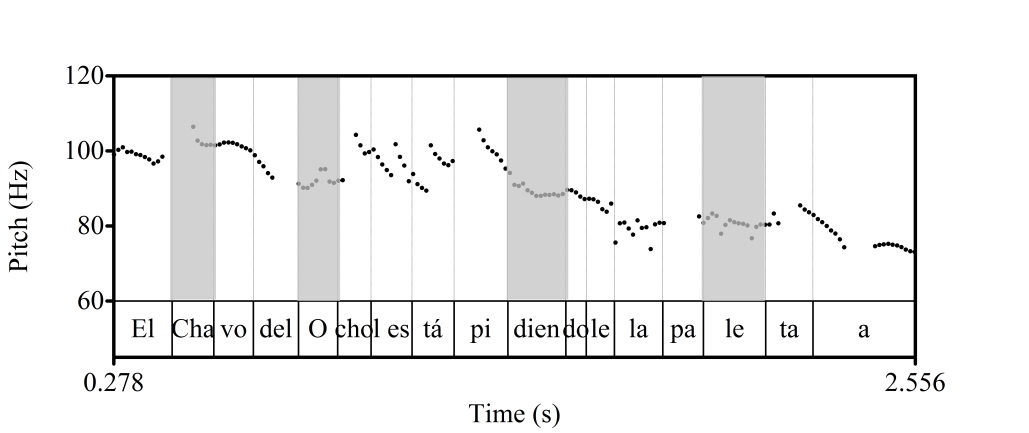
\includegraphics[width=\textwidth]{figures/UTH-img23.png}
 \caption{F0 contour and orthographic transcription of the YS broad focus utterance \textit{El Chavo del Ocho está pidiéndole la paleta a ...} (‘Chavo del Ocho is asking … for the lollipop’, ELIC01/B06\_DMZP)}
\label{fig:uth:1}
\end{figure}

With regard to contrastive focus marking, \citet{Uth16} and \citet{GriceUth15} similarly suggest that contrastive focus is signaled in YS mostly by means of high pitch early in the Intonation Phrase, followed by a fall to the primary stressed syllable of a contrasted word. In many cases, the left high tone is aligned with the left boundary of the Intonation Phrase that contains the contrasted constituent (Figures \ref{fig:uth:2}, \ref{fig:uth:3}).\footnote{Note that the focus particle \textit{sólo} (‘only') in Figures \ref{fig:uth:2} and \ref{fig:uth:4} (i) does not form part of the focus domain in the narrow sense, and (ii) is not known to have any prosodic effect on the latter, except of the fact that it explicitly signals exhaustivity. While we cannot exclude any prosodic effect of this explicit marking of exhaustivity on the focus constituent, it is to be noted that the intonation contours aligned with the relevant stressed syllables do not differ in any way from the further contrastively focused constituents in our YS data.} 

\begin{figure}
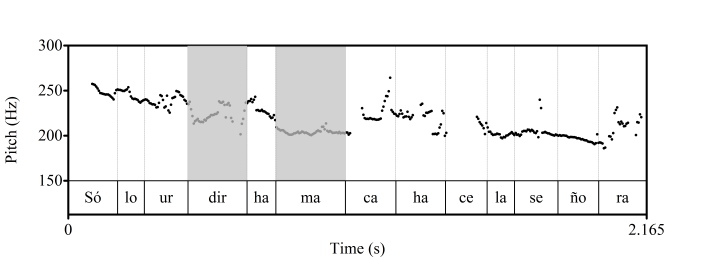
\includegraphics[width=\textwidth]{figures/UTH-img24.png}
 \caption{F0 contour and orthographic transcription of a typical YS verb fronting construction
 \textit{([\textsubscript{F}} \textit{Sólo urdir hamaca] hace la señora}. 
 ‘The only thing the woman does is weave hammocks.’, GJ02/CRA2)}
\label{fig:uth:2}
\end{figure}

\begin{figure}
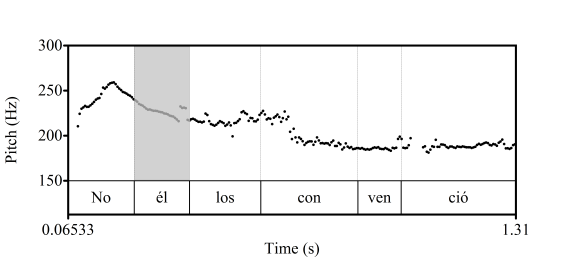
\includegraphics[width=\textwidth]{figures/UTH-img25.png}
 \caption{F0 contour and orthographic transcription of a typical YS construction with negated preverbal contrastive subject 
 ([\textsubscript{F} \textit{No él] los convenció}. 
 ‘It was not him who convinced them.’, GJ02/STE2)}
\label{fig:uth:3}
\end{figure}

In other cases, the high tone does indeed start at the very beginning of the utterance, but extends up to one or two syllables before the contrastive syllable (\figref{fig:uth:4}). 

\begin{figure}
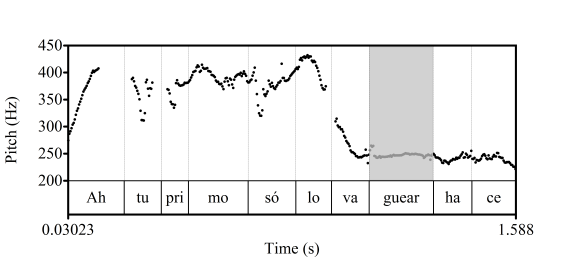
\includegraphics[width=\textwidth]{figures/UTH-img26.png}
 \caption{F0 contour and orthographic transcription of a typical Yucatecan Spanish verb fronting construction 
 (\textit{Ah tu primo, sólo [\textsubscript{F}} \textit{vaguear] hace.}
 ‘Oh, your cousin, all he does is go for walks’; GJ02/CRC2)}
\label{fig:uth:4}
\end{figure}

The difference between YS all-new broad versus contrastive focus marking relates to the overall shape of the utterances' (falling) intonation contours. Accordingly, all-new broad focus utterances such as the one displayed in \figref{fig:uth:1} are characterized by an even, staircase-shaped descent. In contrast, the intonation contour of contrastive focus utterances descends until the last stressed syllable of the contrastive constituent, while the subsequent part of the utterance is generally characterized by a considerable post-focal pitch range compression (Figures \ref{fig:uth:2}--\ref{fig:uth:4}, and cf. below). Moreover, \citet{Uth16} suggests that there are different ways for the speakers to prosodically mark sentence-medial contrastive constituents with left high tones and downward pitch accents. One strategy is to phrase the contrastive constituent separately from the first part of the utterance, so that it aligns with the left edge of ‘its' Intonation Phrase, which usually starts with a initial high tone before declining toward the lexically stressed syllable of the contrastive constituent (\figref{fig:uth:5}). If the corresponding Intonation Phrase includes the preceding auxiliary, the left high tone shifts to the left in order to decline, again, toward the lexically stressed syllable of the contrastive constituent (\figref{fig:uth:6}).
 
\begin{figure}
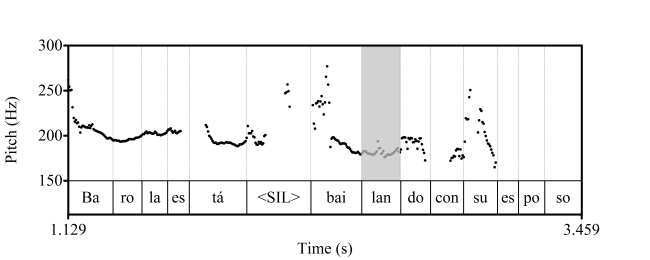
\includegraphics[width=\textwidth]{figures/UTH-img27.png}
 \caption{F0 contour and orthographic transcription of the YS (S)AuxV(XP) sentence 
 \textit{Barola está [\textsubscript{F} bailando] con su esposo}. 
 (‘Barola is dancing with her husband.’, ELIC01/V09\_GGSM)}
\label{fig:uth:5}
\end{figure}

\begin{figure}
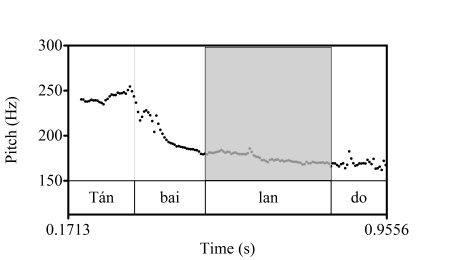
\includegraphics[width=\textwidth]{figures/UTH-img28.png}
 \caption{F0 contour and orthographic transcription of the YS (S)AuxV(XP) sentence
 \textit{Tán [\textsubscript{F}  bailando]}. (…) 
 (`(They) are dancing. (…)', ELIC01/V13\_LYDC)}
\label{fig:uth:6}
\end{figure}

However, we also find utterances whose left high tone extends (or shifts) up to one or two syllables before the contrastive syllable, acting as a leading tone of the corresponding falling pitch accent (\figref{fig:uth:7}). 

\begin{figure}
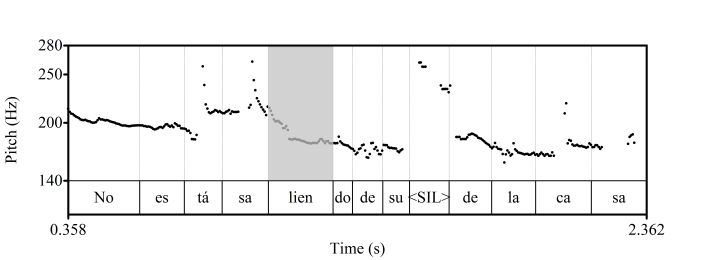
\includegraphics[width=\textwidth]{figures/UTH-img29.png}
 \caption{F0 contour and orthographic transcription of the YS utterance
 \textit{‘No, está [\textsubscript{F} saliendo] de su – de la casa.} 
 ‘No, (she) is leaving her – the house.’, ELIC01/V19\_DMZP)}
\label{fig:uth:7}
\end{figure}

In contrast, speakers of standard Mexican Spanish generally produce the ‘typical’ Spanish contrastive pitch accent L+H* in the corresponding contexts (\figref{fig:uth:8}).

\begin{figure}
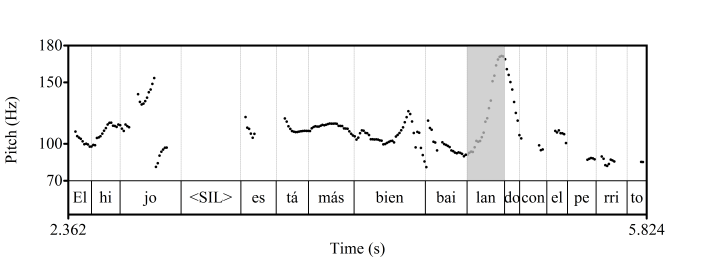
\includegraphics[width=\textwidth]{figures/UTH-img30.png}
 \caption{F0 contour and orthographic transcription of the Mexican Spanish utterance 
 \textit{El hijo está más bien [\textsubscript{F} bailando] con el perrito.} 
 (‘The son is rather dancing with the dog.’, ELIC01/V13\_AHFX)}
\label{fig:uth:8}
\end{figure}

This dialectal difference is especially evident in the realm of contrastive cleft sentences, which commonly exhibit the left high tone followed by falling pitch accents in our YS data (\figref{fig:uth:9}). In the contrastive focused utterances produced by speakers of standard Mexican Spanish, however, the pitch peak is generally aligned at the end of the contrastive syllable (\figref{fig:uth:10}).

\begin{figure}
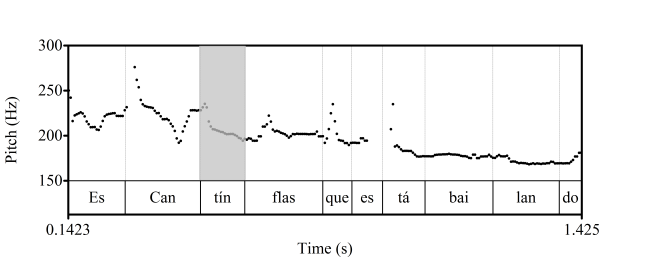
\includegraphics[width=\textwidth]{figures/UTH-img31.png}
 \caption{F0 contour and orthographic transcription of the contrastive cleft sentences \textit{Es [\textsubscript{F}} \textit{Cantínflas] que está bailando}. (‘It is Cantínflas who is dancing.’) in YS}
\label{fig:uth:9}
\end{figure}

\begin{figure}
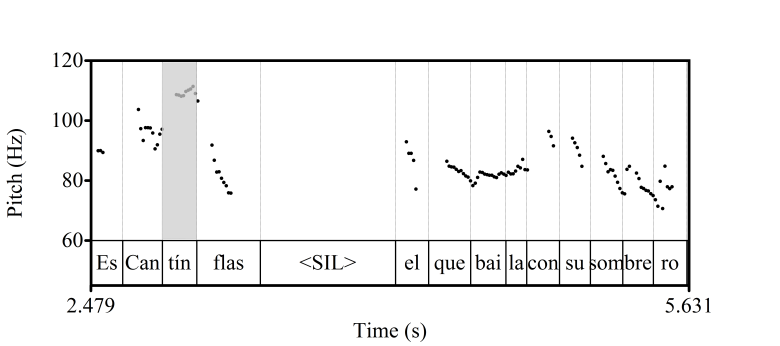
\includegraphics[width=\textwidth]{figures/UTH-img32.png}
 \caption{F0 contour and orthographic transcription of the contrastive cleft sentences 
 \textit{Es [\textsubscript{F} Cantínflas] el que baila con su sombrero}. 
 (‘It is Cantínflas who is dancing with his hat.’) in Standard Mexican Spanish}
\label{fig:uth:10}
\end{figure}

In several cases, such as the contrastive cleft sentence in \figref{fig:uth:9}, the left high tone is followed by a staircase-shaped descent similar to the one that we attested in YS all-new broad focus utterances (cf. \citealt{Uth16}). This is by no means astonishing, since it is a well-known fact that contrastive cleft sentences may, but need not necessarily bear any particular contrastive pitch accent (\citealt[15]{FeldhausenVanrell2015}; \citealt[4298]{MorenoCabrera99}). However, in most of the contrastive cleft sentences analyzed by \citet{Uth16}, the non-clefted part of the utterance still exhibits a considerable post-focal pitch range compression, meaning that it differs from the clefted part (and from broad focus utterances) due to its largely uninflected pitch contour (\figref{fig:uth:11}).

  

\begin{figure}
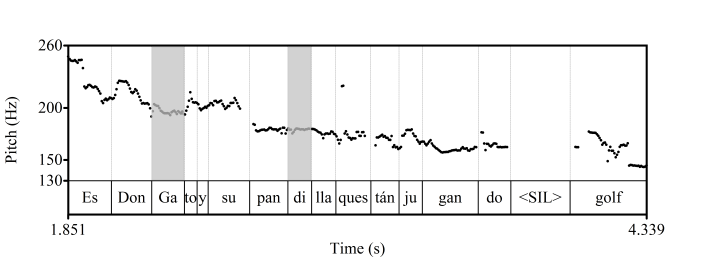
\includegraphics[width=\textwidth]{figures/UTH-img33.png}
 \caption{F0 contour and orthographic transcription of standard YS contrastive cleft sentence 
 \textit{Es [\textsubscript{F} Don Gato y su pandilla] que están jugando golf}. 
 (‘It is Don Gato and his gang who are playing golf.')}
\label{fig:uth:11}
\end{figure}

From a phonological perspective, \citet{GriceUth15} conceive of the YS left high tone as a hybrid tone which originates phonologically as a phrase-marking device but may be attracted by the low(er) tone of the contrastive syllable in order to draw the attention of the listener to the important information. It is important to recall that the left high tone is not restricted to the contrastive domain. On the contrary, YS Intonation Phrases corresponding to all-new broadly focused information are likewise systematically characterized by a left high beginning (cf. again \citealt{Uth16}). This suggests that the YS intonational system is endowed with a left high tone which demarcates the left edge of certain types of intonation units that may (but need not) be exploited by the YS speakers as an attention-orienting device to prepare the listener for upcoming important information (cf. again \citealt{GriceUth15}). 

It should be noted that the particular intonation contours of YS, composed of left high tones and subsequent falling pitch accents, are not to be mistaken for prosodic devices that mark Verum Focus (\citealt{EscandellVidal11}) or rhetorical speech (\citealt{HualdeNadeu13}) in standard European Spanish. Indeed, it is true that the prosodic realization of both of the latter rhetorical devices involves a high peak preceding a low lexically stressed syllable. However, aside from this commonality, the data described by \citet{EscandellVidal11} and \citet{HualdeNadeu13} are clearly different from our YS data. One important difference is that the pragmatic contexts of their data are entirely distinct from the contexts that we investigated in the realm of our investigation of YS sentence prosody. In the instances of Verum Focus analyzed by \citet{EscandellVidal11}, falling pitch accents are used (in sentence-final position) to mark explicitly given information, the main aim being to underline that the information has already been given in prior discourse.  \citet[231]{HualdeNadeu13}, in turn, characterize the prosodic particularity they discern in standard European Spanish rhetorical speech as a ``feature of public speech, when the speaker is speaking to an audience". Moreover, note that both of the abovementioned works treat the prosodic realization of highly confined pragmatic contexts in a (standard) variety of Spanish which is, unlike YS, generally characterized by the predominance of rising pitch accents, especially in contexts of broad and (contrastive) narrow focus realization.

Finally, \citet{Uth17} argues that there are several hints pointing to a possible influence of the contact language, YM, on the above-presented YS intonation patterns. In order to roughly retrace the corresponding line of argument, it is necessary to take into consideration three different findings cited in the literature concerning focus marking in YM. Firstly, it is generally acknowledged that in YM, narrow focus triggers the fronting of the focused constituent to a left-adjacent position of the verb, following the topicalized constituent(s) if there is one/are any (cf. e.g. \citealt{Aissen92,Tonhauser03,GutierrezBravo08,Skopeteas12}). Secondly, \citet{KuglerSkopeteas07} show that the lexical high tones of YM do, in fact, undergo lowering in contrastive contexts. Thirdly, \citet{Verhoeven.2015} trace back the phenomenon of focus fronting to independent prosodic characteristics of YM. Accordingly, YM is a so-called edge language, with the most prominent ‘edge’ being located at the leftmost accented syllable of the Intonational Phrase which is aligned with a left high tone (\figref{fig:uth:23}).

\begin{figure}
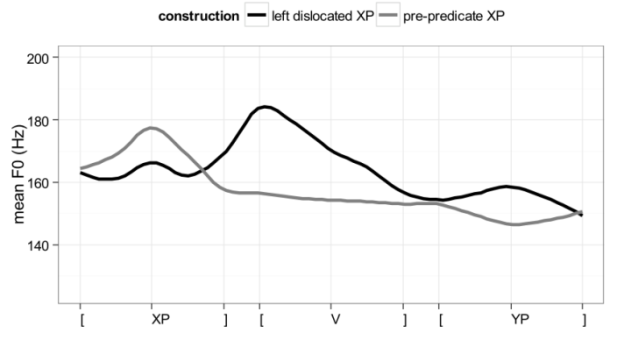
\includegraphics[width=\textwidth]{figures/UTH-img34.png}
\caption{Average tonal contour of [\textsubscript{FOC}XP] -V-XP (grey) and [\textsubscript{TOP}XP] -V-[\textsubscript{FOC}XP] (black) in YM according to \citet{Verhoeven.2015}.}
\label{fig:uth:23}
\end{figure}

This evidence suggests that the fronting of constituents in YM is an instance of leftward ‘p-movement’, which is diametrically opposed to the rightward ‘p-movement’ attested for standard MS by \citet[169]{GutierrezBravoetal17}. Furthermore, the standardized intonational realizations of non-complex sen\-ten\-ces presented by \citet{Verhoeven.2015} suggest that YM intonation is characterized by left high tones and falling intonational contours, very similar to what we revealed above for our YS data.

\section{F0 contours of cleft sentences in the comparative elicitation study}
\label{sec:uth:4}
Concerning the results of our comparative picture-based elicitation experiment, it is to be noted, first of all, that the participants generally behaved in a more natural way in the third condition than in the two conditions designed in analogy to \citet{Gabriel2007}. More precisely, in the third condition, the elicited utterances were remarkably more natural regarding both their prosody (no astonishment, no boredom, no listing intonation) as well as their syntax (greater diversity and shortness of constructions). The participants closely followed the instructions without showing any signs of tiring, distraction, or confusion. Therefore, we can be rather sure that, in the context of the third condition, the participants fully engaged in the ‘game/task’ and faithfully complied with the intended communicative setting. 

In what follows, we will compare designs 1 and 2, which closely follow the design of \citet{Gabriel2007}, with the modified design 3 regarding the prosodic realization of contrastive cleft sentences. (Contrastive) cleft sentences can normally be grouped into one of the following three categories: canonical cleft sentences (\ref{ex:uth:5}a.), pseudo-cleft sentences (\ref{ex:uth:5}b.), and inverted pseudo-cleft sentences (\ref{ex:uth:5}c.).   



\ea\label{ex:uth:5}  
  \ea \gll Fue Aruma la que me dio el diario.\\
      be.past.3sg Aruma who to me give.past.3sg the newspaper\\
      \glt      `It was Aruma who bought the newspaper.'
  \ex \gll  La que me dio el diario fue Aruma.\\
      who to me give the newspaper be.past.3sg Aruma.\\
      \glt  `It was Aruma who gave the newspaper to me.'
  \ex \gll  Blancanieves fue la que lo hizo.\\
      Snow White be.past.3sg who it do.past.3sg\\
	\glt `It was Snow White who did it.'
  \z
\z

\tabref{tab:uth:5} lists the different types of cleft sentences, together with the numbers of occurrence and with labels for the different prosodic realizations of the ‘contrastive syllables', i.e. the lexically stressed syllables of the contrasted constituents attested in our data. In this table, the label H(…)L* refers to the typical YS falling pitch contours described above in \sectref{sec:uth:3} (cf. again Figures \ref{fig:uth:1}-\ref{fig:uth:7}, \ref{fig:uth:9}, \ref{fig:uth:11}). L+H* refers to the ‘contrastive pitch accent' typically found in close-to-standard varieties of Spanish such as e.g. standard Mexican Spanish (cf. again Figures \ref{fig:uth:8}, \ref{fig:uth:10}). L+>H* refers to a pitch accent with a ‘delayed peak', aligned with the syllable that is right-adjacent to the lexically stressed one (cf. \figref{fig:uth:14}). This type of pitch accent is often found in the prefinal parts of broad focus sentences in e.g. standard Mexican Spanish, and other close-to-standard varieties of Spanish (cf. e.g. \citealt{delaMotaetc10}). However, it is important to note that we use these labels in an entirely descriptive, non-phonological way in order to be able to assign each of the individual intonation contours to one of the three attested types.

\begin{table}
\begin{tabularx}{.85\textwidth}{Qrlrl} 
\lsptoprule
& \multicolumn{2}{l}{\bfseries Design 1 \& 2} & \multicolumn{2}{l}{\bfseries Design 3}\\
\midrule 
Canonical                   & 19 & L+>H* & 6 & H(…)L*\\
Pseudo (final S)            & 2  & L+H*  & 2 & H(…)L*, L+H*\\
Inverted pseudo (initial S) & 3  & L+>H* & 1 & L+>H*\\
\midrule
Total                       & 24 &       & 9 & \\
\lspbottomrule
\end{tabularx}
\caption{Number and prosodic realization of different cleft constructions in our comparative picture-based elicitation experiment}
\label{tab:uth:5}
\end{table}

Obviously, the main difference between the data obtained by means of the two different elicitation designs (1 \& 2 versus 3) relates to the falling pitch accents which we described in section 3 to be commonly attested in the context of contrastive focus realization in YS. As evidenced by the figures in \tabref{tab:uth:5}, this particular pitch contour is only attested in the data obtained by means of the more elaborate elicitation design 3. Hence, apart from a minor degree of variation in the context of pseudo-cleft and inverted pseudo-cleft constructions, this data closely adheres to the main characteristics of prosodic focus realization in YS as explained in \sectref{sec:uth:3}. As described for our YS reference corpus in section 3, the left high tones of these contrastive cleft constructions are either realized at the very left edge of the corresponding Intonation Phrase (\figref{fig:uth:12}), or shifts up to one or two syllables before the contrastive syllable, acting as a leading tone of the corresponding falling pitch accent (\figref{fig:uth:13}).\footnote{This utterance is an answer to the contrastive focus question \textit{Es Natalia la que compra el diario en la tienda ¿no?} Note that the corresponding F0 contour does not exhibit any of the common hesitation phenomena (pauses, rising pitch, filler words, or non-modal voice). On the contrary, the speaker has a clear and decisive voice in this example.} As shown in \sectref{sec:uth:3}, both kinds of falling intonation contours are well attested in YS contrastive focus realization.


\begin{figure}
\caption{F0 contour and orthographic transcription of the canonical cleft sentence 
\textit{Fue [\textsubscript{F} Aruma] la que me dio el diario}. 
(‘It was Aruma who gave me the newspaper.’ ELIC02/condition 3/ KEY03\_CS2)}
\label{fig:uth:12}
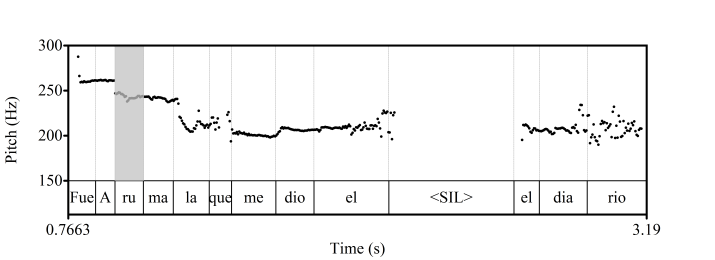
\includegraphics[width=\textwidth]{figures/UTH-img35.png}
\end{figure}

Compared to these data, the ‘contrastive syllables’ obtained by elicitation designs 1 and 2 exhibit very different intonation contours, which can roughly be divided into rising pitch accents with delayed peak (L+>H*) in sentence-initial or sentence-medial position (\figref{fig:uth:14}) and typical standard Spanish contrastive pitch accents' (L+H*) in sentence-final position (\figref{fig:uth:15}). Contrary to what we expected, the falling pitch contours typical of YS are not attested in this part of the data at all.

\begin{figure}
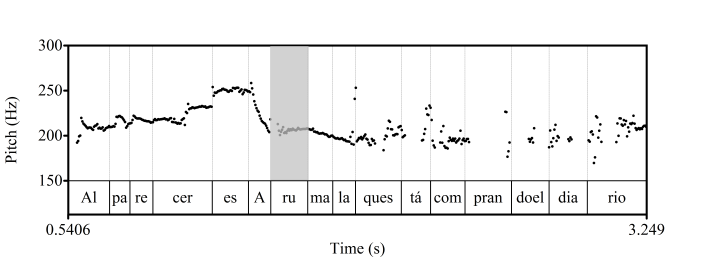
\includegraphics[width=\textwidth]{figures/UTH-img36.png}
\caption{F0 contour and orthographic transcription of the canonical cleft sentence
\textit{Al parecer es [\textsubscript{F} Aruma] la que está comprando el diario}. 
(`It seems that it is Aruma who is buying the newspaper.' ELIC02/condition 3/KEY03\_CS1)}
\label{fig:uth:13}
\end{figure}

Compared to these data, the ‘contrastive syllables' obtained by the elicitation designs 1 and 2 exhibit very different intonation contours, which mainly divide into rising pitch accents with delayed peak (L+>H*) in sentence initial or sentence medial position (\figref{fig:uth:14}), and typical standard Spanish ‘contrastive pitch accents' (L+H*) in sentence final position (\figref{fig:uth:15}). Contrary to what we expected, the falling pitch contours typical for YS are not attested in this part of the data at all.

\begin{figure}
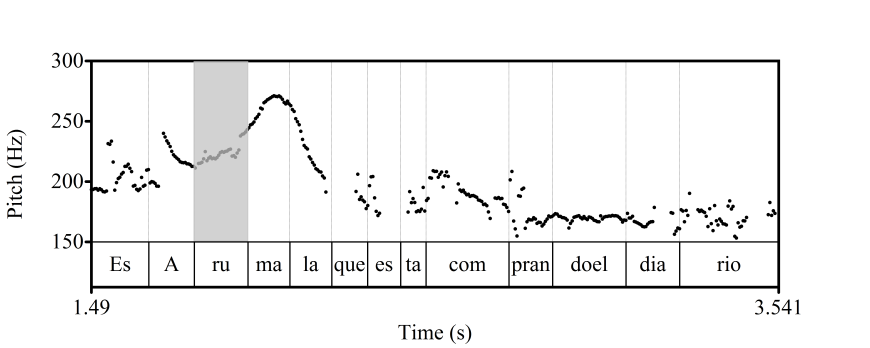
\includegraphics[width=\textwidth]{figures/UTH-img37.png}
\caption{F0 contour and orthographic transcription of the canonical cleft sentence \textit{Es [\textsubscript{F}} \textit{Aruma] la que está comprando el diario}. (‘It is Aruma who is buying the newspaper', ELIC02/condition 1/ZAY01\_CS1)}
\label{fig:uth:14}
\end{figure} 
 
\begin{figure}
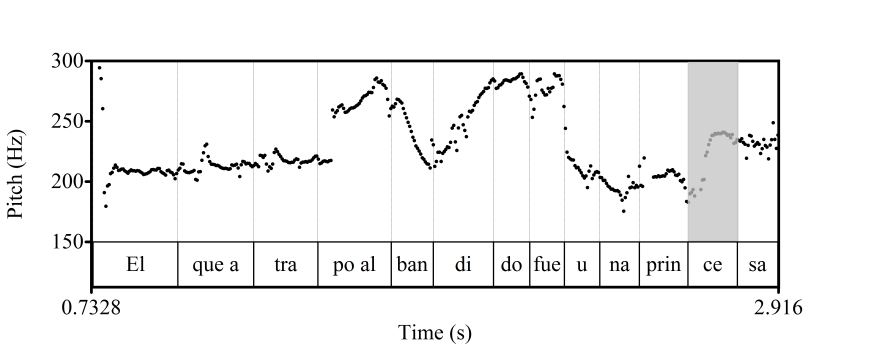
\includegraphics[width=\textwidth]{figures/UTH-img38.png}
\caption{F0 contour and orthographic transcription of the pseudo-cleft sentence \textit{El que atrapó al bandido fue una [\textsubscript{F}} \textit{princesa]} (‘It was a princess who captured the bandit.' ELIC02/condition 2/KEM02\_CS3)}
\label{fig:uth:15}
\end{figure}

In view of the fact that all the participants in the comparative elicitation experiment were monolingual speakers of YS, it is hard to interpret the deviant intonation contours obtained by elicitation designs 1 and 2 in a meaningful way. According to our analysis of YS sentence prosody described in \sectref{sec:uth:3}, the participants in conditions 1 and 2 ‘should' normally produce falling intonation contours similar to the ones in condition 3, but obviously they do not do so.

Having said this, it is obvious that the two sentence-final L+H* pitch accents may be attributed to inner- or intra-speaker variation, which is common for a Spanish contact variety such as YS. Moreover, note that we also find one instance of this pattern in the data obtained in design 3. However, intonation contours such as the one displayed in \figref{fig:uth:14} are not attested in the latter sub-corpus. In order to account for this kind of intonation contour, we need to present some more details concerning the analysis of broad focus sentences alluded to in \sectref{sec:uth:3}. 

It is true that YS Intonation Phrases which correspond to all-new broadly focused information seem to be generally characterized by a left high beginning followed by one or more falling pitch accents (cf. again \figref{fig:uth:1}). However, this intonation contour is not the only one, and not even the most frequent one, attested in the context of broad focus elicitation by \citet{Uth16}. In contrast, the majority of the broad focus utterances extracted from the elicitation data produced by the YS speakers cited in \citet{Uth16} are characterized by the following functional division: Subjects are mostly realized with a rising pitch accent, whereas the subsequent parts of the utterances are uniformly realized by falling pitch contours (Figures \ref{fig:uth:16}, \ref{fig:uth:17}).

\begin{figure}
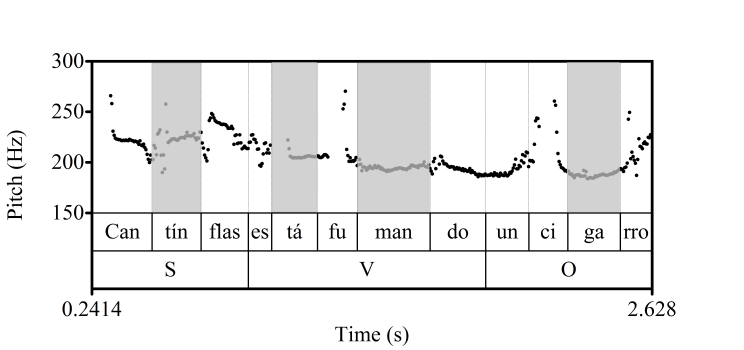
\includegraphics[width=\textwidth]{figures/UTH-img39.png}
\caption{F0 contour and orthographic transcription of the Yucatecan Spanish broad focus sentence \textit{Cantínflas está fumando un cigarro}.
(‘Cantinflas is smoking a cigarette.' ELIC01/B20\_GGSM)}
\label{fig:uth:16}
\end{figure}

Interestingly, \citet{MartinButraguenoetal15} also attest early aligned peaks in prenuclear position based on data by 9 mostly monolingual YS speakers from Mérida who performed semi-spontaneous elicitation experiments and reading tasks on the basis of the elicitation materials designed by the teams of AMPER and IARI.\footnote{AMPER = \textit{Atlas Multimedia de la Prosodia del Espacio Románico} < \url{http://stel.ub.edu/labfon/amper/}> [29.12.2015];
IARI = Interactive Atlas of Romance Intonation <\url{http://prosodia.upf.edu/iari/} >[29.12.2015].} However, they concomitantly indicate that (i) the final stressed syllable in a typical YS utterance is low (L*) or downstepped high (!H*, ``descenso yucateco{\textquotedbl}, ‘Yucatecan fall', \citealt{MartinButraguenoetal15}), and (ii) the pitch contour following the first peak is likewise very often descending. Another interesting aspect of their research has to do with the proportions of different pitch accent types depending on the position of the lexically stressed syllables in the sentence. Their data exhibit an overwhelming amount of downstepped high pitch accents in second, third, and fourth accent position, whereas the initial lexically stressed syllables are mostly associated with rising pitch accents. 

Our results are in line with \citet{MartinButraguenoetal15} inasmuch as the non-rising pitch movements in the data analyzed by \citet{Uth16} might equally be analyzed as downstepped high and low pitch accents, depending on their exact intonational realization and their position in the sentence. Interestingly, \citet{MartinButraguenoetal15} reveal that the typically Yucatecan downstepped high and low pitch accents are predominantly attested from the second lexically stressed syllable onwards (with 50--64\% downstepped high pitch accents), whereas the first lexically stressed syllable is often (up to 52\%) realized by rising pitch contours.  

However, in the data described by \citet{Uth16}, the divide between rising and non-rising pitch movements seems to be related to the functional difference between subject constituents (with a varying number of lexically stressed syllables) and non-subject constituents, rather than accent position (cf. \figref{fig:uth:17}). Furthermore, the following two pieces of evidence suggest that the corresponding subject constituents are treated as given, or even topicalized information by the participants, whereas the subsequent parts of the utterances correspond to (virtually) new information. Firstly, the elicitation design used by \citet{Uth16} provides a communicative setting in which the referents are introduced into the discourse by means of accompanying pictures, which furthermore often display the referents' names in order to obtain utterances that are comparable inter-individually. Secondly, the subject constituents are often phrased separately from the rest of the utterances, as indicated by the high number of pauses following the subject constituent (cf. again \figref{fig:uth:17}).
 
\begin{figure}
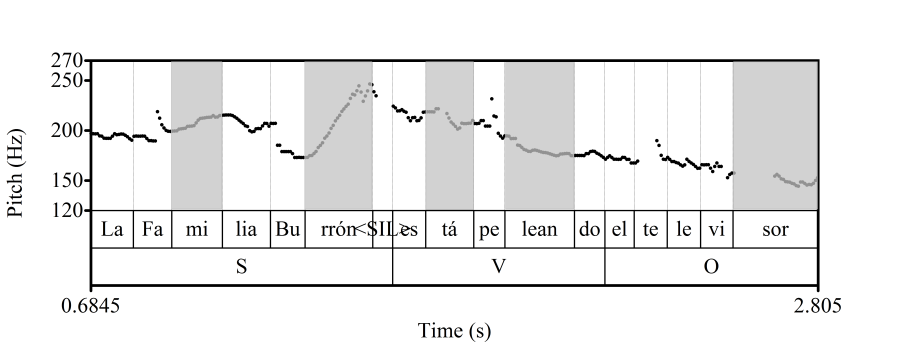
\includegraphics[width=\textwidth]{figures/UTH-img40.png}
\caption{F0 contour and orthographic transcription of the Yucatecan Spanish broad focus sentence 
\textit{La Familia Burrón está peleando el televisor} 
(‘The Burrón Family is fighting over the television.’ ELIC01/B18\_DMZP)}
\label{fig:uth:17}
\end{figure}

Against this background, we suggest that the deviant intonation contours of the contrastive cleft sentences obtained by means of elicitation designs 1 and 2 do not constitute a case of prosodic (contrastive) focus marking at all. Rather, the rising intonation contours at the beginning of the contrastive cleft sentences obtained by designs 1 and 2 should be interpreted similarly to the above-mentioned ‘broad focus' data cited in \citet{Uth16}. More precisely, the hypothesis is that the participants confronted with materials 1 and 2 do not properly contrast the referents as intended, but rather use the cleft constructions in a non-contrastive context, similarly to what \citet[4299]{MorenoCabrera99} and \citet{FeldhausenVanrell2015} suggest with respect to pseudo-cleft sentences and inverse pseudo-cleft sentences in standard European Spanish. According to this approach, the rising contours at the beginning of the utterances of conditions 1 and 2 are due to the fact that the subject constituents correspond to given information which was introduced into the discourse at the very beginning of the elicitation task.

From a phonological viewpoint, it could be argued that this partitioning of Information Structure is indicated in YS by means of a high intermediate phrase boundary (H-) at the end of the given/topicalized constituent. This is especially evident in several cleft sentences which include a second intermediate phrase boundary, presumably due to the fact that all linguistic material preceding this boundary is treated as given (\figref{fig:uth:18}). However, the phonological analysis of this data is beyond the scope of the present paper. Therefore, we content ourselves with the descriptive observation of the predominant L+>H* contour at the beginning of the canonical cleft sentences of conditions 1 and 2, which is highly reminiscent of the above-mentioned ‘broad focus' data, irrespective of any phonological analysis. 


\begin{figure}
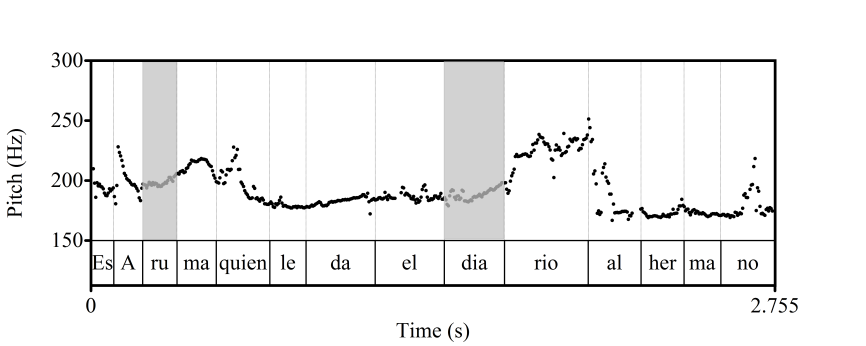
\includegraphics[width=\textwidth]{figures/UTH-img41.png}
\caption{F0 contour and orthographic transcription of the canonical cleft sentence 
\textit{Es [\textsubscript{F}} \textit{Aruma] quien le da el diario al hermano}. 
(‘It is Aruma who gives the newspaper to her brother', ELIC02/condition 1/DOR01\_CS2)}
\label{fig:uth:18}
\end{figure}

It is true that the exact interpretation of the above-cited data is a matter of debate and the exact relationship between propositional attitudes, illocutionary acts, and information structural categories are far from being clear yet – let alone the proportional prosodic effects of all of these different pragmatic categories in natural speech (cf. \citealt{Reich17}). However, the important point for the present purpose is that the intonational realization of the cleft constructions which we obtained by means of our comparative elicitation experiment seems to depend on the exact design of the elicitation material. We consider this difference in intonational realization to be further evidence of the need for more elaborated contexts and unequivocal triggers in the realm of focus elicitation. 

\section{Conclusions}
\label{sec:uth:5}
In this paper, we discussed the design of semi-spontaneous picture-based elicitation experiments for eliciting the syntactic and prosodic realization of different focus types (broad, narrow, and contrastive) in Spanish. In doing so, we took a rather skeptical position with regard to the reach of the pragmatic control of some picture- and short story-based elicitation materials. It is argued that the corresponding designs contain several pragmatic mismatches which might impede the participants from properly performing the language task as intended, meaning that there are good reasons to doubt that the corresponding production data can be unambiguously coded for pragmatic contexts and/or propositional attitudes. However, propositional attitudes have been revealed to highly influence the prosodic realization of questions and assertions in different languages. Thus, it might be reasonable to stick to elicitation designs with concrete and explicit communicative settings in order to be able to control as closely as possible for the attitudes of the participants toward the propositional content of their utterances. 

In a second step, the paper reported on a comparative picture-based elicitation experiment based on Yucatecan Spanish and composed of three designs which differ slightly with respect to the pragmatic appropriateness of the picture stimuli and the accompanying questions. Our analysis of the production data obtained by means of these materials suggests, among other things, that (at least) for Yucatecan Spanish contrastive cleft sentences the intonational realization of the constructions also depends on the exact design of the elicitation experiment. It is argued that this difference in intonational realization should be conceived as further evidence of the need for more elaborated contexts and unequivocal triggers in the realm of focus elicitation. 

{\sloppy
\printbibliography[heading=subbibliography,notkeyword=this]
}

\end{document}